
\subsection{Comportamientos e implementaciones}
\label{comportamientos}

Una vez que decidimos utilizar la arquitectura explicada en la secci\'on \ref{arq_prop}
para nuestro proyecto, tuvimos que analizar:
\begin{itemize}
\item{}Forma de implementaci\'on de la arquitectura en c\'odigo
\item{}Comportamientos a realizar
\item{}Ordenes de inhibici\'on y supresi\'on entre los mismos
\item{}Forma de implementaci\'on de los mismos
\item{}Orden de implementaci\'on
\end{itemize}

%Detallar que se hizo con cada item
Para implementar la arquitectura decidimos asignarle un $ID$ num\'erico diferente a cada comportamiento.
Tambi\'en tomamos la decisi\'on de elegir como comportamiento activo en el instante $t$,
aquel comportamiento que est\'e activo en ese instante y tenga mayor $ID$,
suprimiendo as\'i el resto de los comportamientos ( con un $ID$ menor ) que podr\'ian estar activos.

%Explicar como se relaciona el requerimiento (robot recolector de basura autonomo) con los comportamientos que pusimos
El requerimiento de este proyecto es la realizaci\'on de un robot aut\'onomo que recolecte
basura de su entorno din\'amico pero estructuralmente fijo. De aqu\'i se infieren algunos de los
comportamientos que debe tener el robot:
\begin{itemize}
	\item{\emph{Recolectar basura} (\ref{collect_garbage})}
	\item{\emph{Recargar bater\'ia} (\ref{recharge_battery}):} Por ser aut\'onomo, debe poder 
			ser capaz de recargarse s\'olo para poder continuar con su actividad.
	\item{\emph{Wandering} (\ref{wandering}):} El robot no es controlado por control, ya que
			es aut\'onomo, por lo que debe poder recorrer el entorno por s\'i mismo.
	\item{\emph{Evitamiento de obst\'aculos} (\ref{avoid_obstacles}):} Debido a la naturaleza del
			entorno, el robot debe ser capaz de navegar sin chocarse contra los l\'imites del entorno
			ni con las personas que circulan por el mismo.
\end{itemize}

El comportamiento de recolectar basura y el requerimiento de la autonom\'ia llevan a su vez
a la aparici\'on de m\'as comportamientos: \emph{Descargar basura} (\ref{unload_garbage})
e \emph{Ir hacia basura} (\ref{go_to_garbage}).
\\
La figura \ref{fig:architecture} muestra los comportamientos implementados y su orden de jerarqu\'ia.
Se puede ver que hay m\'as comportamientos de los detallados anteriormente. \'Esto se debi\'o a que la forma
en que se implementamos los comportamientos b\'asicos del robot nos requiri\'o el desarrollo
de comportamientos auxiliares.
\\
\begin{figure}[htp]
\begin{center}
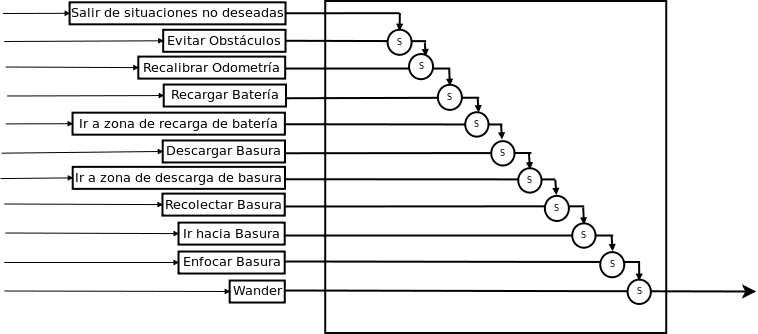
\includegraphics[scale=0.5]{comportamientos/behavioursArchitecture2.png}
\caption{Arquitectura de Comportamientos}
\label{fig:architecture}
\end{center}
\end{figure}
\\
Primero implementamos \emph{Wandering} debido a, en una primera aproximaci\'on, la sencillez
del mismo. Luego implementamos \emph{Evitamiento de obst\'aculos} para lograr que el robot pueda
navegar sin problemas por el arena. Como el comportamiento de recolectar e ir hacia la basura
dependend\'ia del m\'odulo de reconocimiento de objetos y el mismo estaba siendo desarrollado
en paralelo, se decidi\'o implementar el comportamiento de \emph{Recargar bater\'ia} y \emph{Descargar basura}.
Una vez que tuvimos la primera implementaci\'on funcional del reconomiento de objetos, procedimos a
desarrollar \emph{Ir hacia basura} y \emph{Recolectar Basura}.
\\
A continuaci\'on detallamos los comportamientos indicados en la figura \ref{fig:architecture},
as\'i como la implementaci\'on en \textit{pseudo-codigo} de los mismos y detalles tenidos
en cuenta para la realizaci\'on de los mismos.
%A continuacion vamos a explicar cada comportamiento.....

\subsubsection{Wandering}
\label{wandering}

\paragraph{Detalle del comportamiento} 
Por ser el comportamiento que menor jerarqu\'ia tiene (Ver \ref{fig:architecture}), es el \'unico
comportamiento que est\'a activado ante la ausencia de un est\'imulo, asegurandonos que siempre
haya por lo menos un comportamiento activo.
\\
En una primer aproximaci\'on de \emph{Wandering}, s\'olo nos preocupamos por ir hacia adelante
ya que eventualmente, el robot encuentra un obst\'aculo y realiza un giro cambiando la direcci\'on
del robot.
\\
Los resultados de la simulaci\'on nos indicaron que el robot no recorr\'ia ciertas zonas o las recorr\'ia
despu\'es de un largo tiempo, lo que nos llev\'o a un segundo approach. El mismo tiene en cuenta el hecho
de que el robot posee una c\'amara y por lo tanto se puede llevar un seguimiento de los lugares que m\'as
recientemente visit\'o o las zonas que hace mucho tiempo no visita.
\\
\'Este approach, en cierta forma, genera un modelo del mundo, un hecho que conflict\'ua con uno de
los principios propuestos a seguir en la secci\'on \ref{arq_prop}. Para minimizar el conflicto, decidimos
mantener al m\'inimo la informaci\'on almacenada para el funcionamiento del algoritmo, es decir, por cada
zona de arena s\'olo mantenemos el timestamp de la \'ultima vez que el robot la visit\'o.

\paragraph{Implementaci\'on del comportamiento}

La implementaci\'on del segundo approach, en \emph{pseudo-c\'odigo} es la siguiente:
\begin{verbatim}
por cada paso
    zona = pedir_zona_vista(camara)
    marcar_zona_como_vista(modelodelmundo,zona)
    ultimazonavisitada = pedir_ultima_zona_visitada(modelodelmundo)
    velocidades = calcular_velocidades_de_ruedas(ultimazonavisitada)
    poner_velocidades_en_ruedas(velocidades)
\end{verbatim}
Para obtener la zona vista por la c\'amara, necesitamos de la altura $C_h$ a la cual est\'a ubicada
la c\'amara en el robot, el campo de visi\'on (de ahora en adelante \emph{Field of View o FOV})
horizontal $FOV_h$ o vertical $FOV_v$ y el \'angulo de inclinaci\'on de la c\'amara $ac$. Viendo la figura
\ref{fig:angleCamera} podemos ver que:

\begin{figure}[htp]
\begin{center}
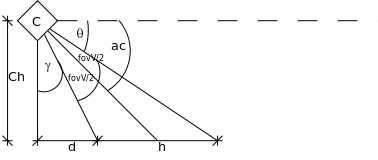
\includegraphics{comportamientos/angleCamera.png}
\caption{Diagrama de posici\'on de la c\'amara}
\label{fig:angleCamera}
\end{center}
\end{figure}

\begin{eqnarray}
ac + \frac{FOV_v}{2} + \gamma = \frac{\pi}{2}\\
\gamma + FOV_v + \theta = \frac{\pi}{2}\\
\tan(\gamma) = \frac{d}{C_h}\\
\tan(\gamma+FOV_v) = \frac{d+h}{C_h}
\end{eqnarray}

%En caso de no disponer del $FOV_v$, el mismo se puede obtener de:
%\begin{equation}
%FOV_v = \atan(\frac{ \tan(\frac{FOV_h}{2}) * height}{width} * 2)\\
%\end{equation}
Organizando las ecuaciones, podemos deducir que:

\begin{eqnarray}
\gamma = \frac{\pi}{2} + ac - \frac{FOV_v}{2}\\
\label{eqn:distance_d}
d = \tan(\gamma) * C_h \\
\label{eqn:distance_dh}
d+h = \tan(\gamma+FOV_v) * C_h
\end{eqnarray}

Por lo que obtenemos el \'angulo hasta el inicio de la im\'agen de la c\'amara $\gamma$ y como consecuencia,
la distancia $d$ desde la posici\'on de la c\'amara hasta el inicio de la im\'agen y $d+h$,
la distancia desde la posici\'on de la c\'amara hasta el final de la im\'agen. Usando \'estos
datos, la posici\'on del robot $P$ y bas\'andonos en la figura \ref{fig:zoneCamera}, podemos obtener
los puntos $A$, $B$, $C$ y $D$ del trapezoide que determina la zona que ve la c\'amara.

\begin{figure}[htp]
\begin{center}
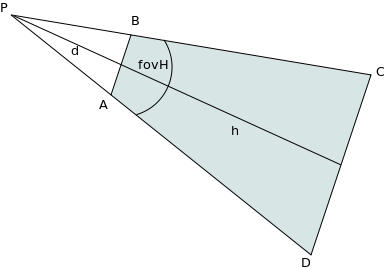
\includegraphics[scale=0.5]{comportamientos/rectangleWander.png}
\caption{Zona vista por la c\'amara}
\label{fig:zoneCamera}
\end{center}
\end{figure}

\subsubsection{Enfocar Basura}
\label{focus_garbage}
Una vez que el m\'odulo de detecci\'on de objetos reconoce algo como basura
(ver secci\'on \ref{algoritmo_vision}), hay que elegir
la forma en que se va a la basura. En la figura \ref{fig:papproachgoto} se puede ver un
primer approach de hacer \'esto. Consiste en primero enfocar la basura de forma tal que
la misma quede en el centro de la imagen de la c\'amara. De aqu\'i surge el comportamiento
\emph{Enfocar Basura}.
\\
Un segundo approach (Figura \ref{fig:sapproachgoto}) no consiste en enfocar la basura,
sino que se idea un arco hacia la misma. \'Esto requiere que se seteen las velocidades
correspondientes a las ruedas de forma tal que la trayectoria del robot describa dicho
arco. Con este segundo approach no existir\'ia el comportamiento que se est\'a describiendo.
\\
Dado que el primer approach es levemente m\'as simple de implementar, y teniendo en cuenta el
principio enunciado en la secci\'on \ref{arq_prop} \emph{``La simplicidad es una virtud''},
elegimos implementar el mismo, a pesar de tener un posible inconveniente, como se puede
ver en la figura \ref{fig:papproachgotoproblem}.
\\
Cuando hay una basura en alguna esquina
superior de la imagen de la c\'amara, y el robot gira sobre s\'i mismo para enfocarla,
la basura puede llegar a perderse por el fondo de la imagen. \'Esto se debe a que la distancia
hacia dichas esquinas es mayor a la distancia hacia el centro del borde superior de la imagen
(Ver figura \ref{fig:zoneCamera}). Decimos que es un ``posible'' problema, ya que una vez que se
pierde de vista la basura, el robot no enfocar\'a m\'as debido a que el est\'imulo desapareci\'o,
pero si luego se dirige hacia adelante (por la activaci\'on de alg\'un otro comportamiento), 
la basura volver\'a a aparecer en la imagen, sin desaprovechar la oportunidad de recogerla.

\begin{figure}[htp]
\begin{center}
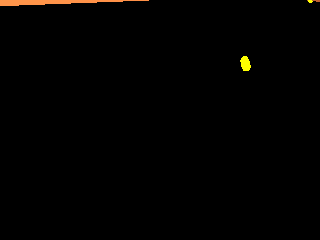
\includegraphics[scale=0.5]{comportamientos/basura.png}
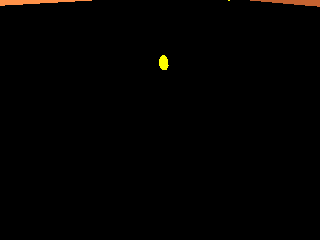
\includegraphics[scale=0.5]{comportamientos/basuraenfocada.png}
\caption{Primer approach de ir a la basura}
\label{fig:papproachgoto}
\end{center}
\end{figure}

\begin{figure}[htp]
\begin{center}
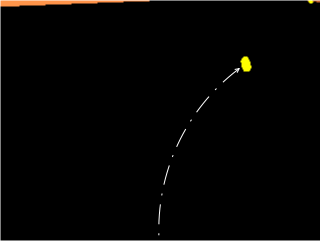
\includegraphics[scale=0.5]{comportamientos/basuraAlt.png}
\caption{Segundo approach de ir a la basura}
\label{fig:sapproachgoto}
\end{center}
\end{figure}

\begin{figure}[htp]
\begin{center}
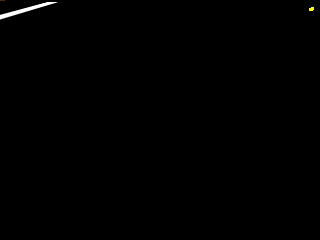
\includegraphics[scale=0.3]{comportamientos/esquina.png}
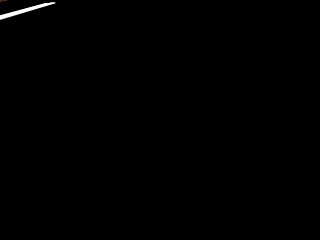
\includegraphics[scale=0.3]{comportamientos/frentemuylejos.png}
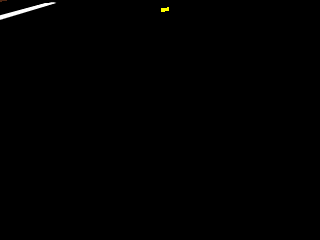
\includegraphics[scale=0.3]{comportamientos/frentelejos.png}
\caption{Posible inconveniente con el primer approach de ir a la basura}
\label{fig:papproachgotoproblem}
\end{center}
\end{figure}

\paragraph{Detalle del comportamiento}
El approach elegido, entonces, se puede describir como:
\begin{itemize}
\item Si la basura est\'a a la izquierda de la im\'agen, se debe girar hacia la izquierda
\item Si la basura est\'a a la derecha de la im\'agen, se debe girar hacia la derecha
\item Si la basura est\'a en el centro, ya est\'a enfocada
\end{itemize}

%En el caso que haya m\'as de una basura elegimos la m\'as cercana, usando c\'alculos
%detallados a continuaci\'on.
\paragraph{Implementaci\'on del comportamiento}
\label{focus_garbage:impl}
El comportamiento sigue el siguiente \emph{pseudo-codigo}:
\begin{verbatim}
por cada paso
    lista_de_basuras = obtener_lista_de_basuras(modulodereconocimiento)
    basura_mas_cercana = elijo_basura_mas_cercana(lista_de_basuras)
    angulo_a_basura = obtener_angulo(basura_mas_cercana)
    velocidad = VELOCIDAD_BASE * ( abs(angulo_a_basura) / (PI/2) )
               + VELOCIDAD_BASE_MINIMA

    si angulo_a_basura < 0 entonces
        veloc_izq = -velocidad
        veloc_der = velocidad
    sino
        veloc_izq = velocidad
        veloc_der = -velocidad
    fin_si
    poner_velocidades_en_ruedas(veloc_izq,veloc_der)
\end{verbatim}

Se puede ver que la velocidad de giro del robot es proporcional al m\'odulo del \'angulo
que hay hacia la basura, logrando enfocar m\'as r\'apido cuando el \'angulo es mayor y
tener mayor precisi\'on cuando el \'angulo es m\'as chico, adem\'as de tener mayor rapidez
de enfoque y precisi\'on que si la velocidad de giro fuera constante.
\\

%%Para obtener el \'angulo y distancia hacia una basura....
%%pasamos de una posicion (x,y) en la imagen a una posicion
%(x,z) en el mundo. teniendo nuestra posicion P, podemos
%calcular la distancia y el angulo
\subsubsection{Ir a Basura}
\label{go_to_garbage}
Luego de la elecci\'on de la forma que se resuelve la situaci\'on de encontrar una
basura (ver \ref{focus_garbage}), el comportamiento de ir a basura es trivial, ya
que la basura, luego de ser enfocada, est\'a delante del robot y lo \'unico que
basta es ir hacia adelante.

\paragraph{Detalle del comportamiento}
El est\'imulo necesario para que este comportamiento est\'e presente est\'a
dado por dos condiciones:
\begin{enumerate}
\item El m\'etodo de reconociemiento de objetos reconoci\'o una basura
\item La basura se encuentra en un entorno del medio horizontal de la imagen de la c\'amara
\end{enumerate}

\paragraph{Implementaci\'on del comportamiento}
\label{go_to_garbage:impl}
\begin{verbatim}
por cada paso
    distancia = obtener_distancia_a_basura(modulodereconocimiento)
    coeff = (distancia - DIST_MIN)/(DIST_MAX - DIST_MIN)
    veloc_der = VELOCIDAD_MIN*(1 - coeff) + coeff*VELOCIDAD_MAX
    veloc_izq = veloc_der
    poner_velocidades_en_ruedas(veloc_izq,veloc_der)
\end{verbatim}

Al igual que en la implementaci\'on del comportamiento \ref{focus_garbage:impl},
las velocidades que se le otorgan a las ruedas dependen de la distancia
hacia la basura, de forma tal que si una basura est\'a muy lejos, la velocidad
sea mayor y a medida que se va acercando, vaya disminuyendo linealmente.

Dado que la basura se encuentra en un entorno del eje Y en la imagen (Ver figura
\ref{fig:image_coord_conv}b) cometemos un error muy peque\~no al estimar la distancia
a la basura como si estuviera sobre el mismo (asumiendo que la coordenada X de la
basura en la imagen es 0).

Como muestran las figuras \ref{fig:image_coord_conv} y \ref{fig:angleCamera},
el \'angulo vertical hacia el punto m\'as alto de la imagen $(0,C_{rh})$ es 
$\gamma+FOV_v$ y hacia el m\'as bajo, $(0,0)$, el \'angulo es $\gamma$.
De las ecuaciones \eqref{eqn:distance_d} y \eqref{eqn:distance_dh} sabemos
las distancias a los puntos $(0,0)$ (DIST\_MIN) y $(0,C_{rh})$ (DIST\_MAX). 
Entonces, para obtener la distancia $dy$ hacia el punto $(0,y)$ basta con
calcular:
\begin{eqnarray}
y_{angle} = FOV_v * \frac{y}{h} \\
dy = \tan(\gamma + y_{angle}) * C_h \\
\end{eqnarray}

donde $y_{angle}$ es la proporci\'on de $FOV_v$ hacia $y$.
\begin{figure}[htp]
\begin{center}
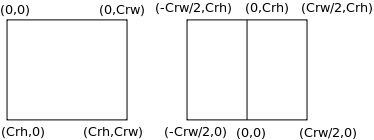
\includegraphics[scale=0.5]{comportamientos/imageCoordsConvertion.png}
\caption{Conversi\'on de coordenadas de imagen de c\'amara}
\label{fig:image_coord_conv}
\end{center}
\end{figure}

\subsubsection{Recolectar Basura}
\label{collect_garbage}
Una vez que el robot llego a estar posicionado para recolectar la basura deseada,
el comportamiento de \emph{recolectar basura} se activa. El mecanismo para \'esto
fue cambiando a lo largo del desarrollo del proyecto.
\\
En un principio pensamos en usar una rampa interna dentro del robot, de forma
tal que la basura suba esa rampa para luego caer en un dep\'osito de basura
interno al robot. Por problemas con la simulaci\'on de este procedimiento, se
busc\'o otro mecanismo.
\\
El mecanismo que elegimos para usar en la simulaci\'on fue el siguiente:
\begin{itemize}
	\item El robot tiene un servo en su parte posterior (debajo de la c\'amara)
	\item Dos paredes delimitan el espacio a lo largo de la direcci\'on que une
			el centro del robot con el servo anteriormente mencionado.
\end{itemize}

\paragraph{Detalle del comportamiento}
La activaci\'on de \emph{recolectar basura} depende de 3 condiciones:
\begin{itemize}
	\item Las dos condiciones impuestas para \emph{ir a basura}
	\item La distancia a la basura elegida para ser recolectada debe ser menor a
			un umbral.
\end{itemize}

Aqu\'i se puede observar que tan importantes son los comportamientos anteriores
para que el robot logre recolectar la basura.
\\
Es importante la elecci\'on del umbral: un valor muy chico puede llevar a que el
comportamiento no se active porque la basura ya no est\'a m\'as en la imagen. Por
otro lado, un valor muy grande causar\'ia que el robot se disponga a recolectar 
una basura que est\'a muy lejos y podr\'ia llegar a moverse por cuestiones propias
del ambiente, llevando as\'i a una innecesaria activaci\'on del comportamiento.

\paragraph{Implementaci\'on del comportamiento}
El \emph{pseudo-codigo} de este comportamiento es el siguiente:

\begin{verbatim}
    distancia = obtener_distancia_a_basura(modulodereconocimiento)
    levantar(servo_delantero)
    recorrerdistancia(distancia)
    cerrar(servo_delantero)
\end{verbatim}

La distancia hacia la basura es obtenida de la misma forma que en la secci\'on
\ref{go_to_garbage:impl}. Levantar y cerrar el servo consiste en setear su
posici\'on en $\frac{\pi}{2}$ y $0$ respectivamente. Para calcular la distancia
recorrida se utiliz\'o la distancia entre la posici\'on del robot en el instante $t$,
$P_r(t)$ y el instante $t+1$, $P_r(t+1)$, ambas dadas por la odometr\'ia
(Ver secci\'on \ref{odometry}). Las diferentes etapas de la recolecci\'on de una
basura se puede ver en la figura \ref{fig:recollection}.

\begin{figure}[htp]
\begin{center}
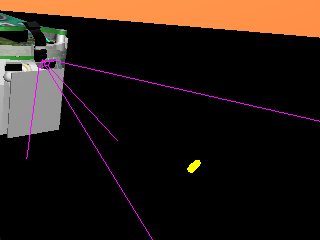
\includegraphics[scale=0.25]{comportamientos/collect1.png}
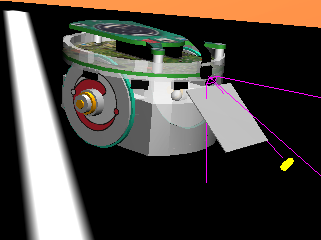
\includegraphics[scale=0.25]{comportamientos/collect2.png}
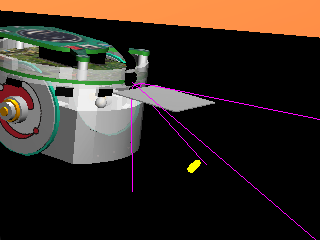
\includegraphics[scale=0.25]{comportamientos/collect3.png}
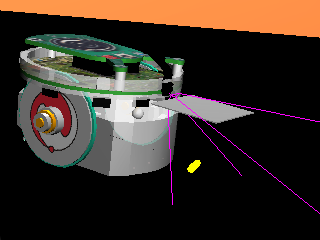
\includegraphics[scale=0.25]{comportamientos/collect4.png}
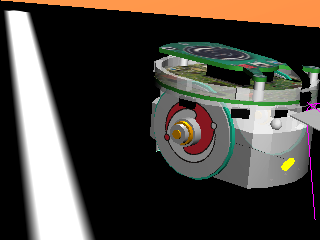
\includegraphics[scale=0.25]{comportamientos/collect5.png}
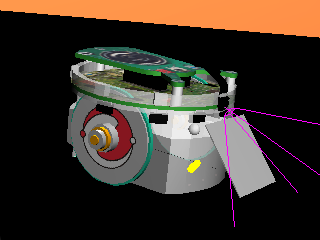
\includegraphics[scale=0.25]{comportamientos/collect6.png}
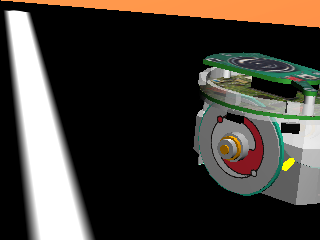
\includegraphics[scale=0.25]{comportamientos/collect7.png}
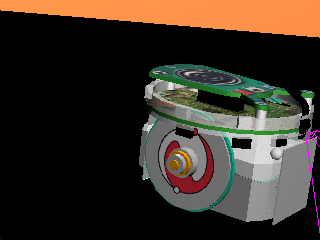
\includegraphics[scale=0.25]{comportamientos/collect8.png}
%
\includegraphics[scale=0.3]{comportamientos/unk.jpg}
\caption{Etapas de recolecci\'on de basura}
\label{fig:recollection}
\end{center}
\end{figure}


\subsubsection{Ir a zona de descarga de basura}
\label{go_to_unload_zone}
Como la capacidad del dep\'osito interno de basura del robot tiene un l\'imite, 
surge como necesidad que el robot sea capaz de ir hacia una zona donde descargar\'a
la basura que contiene, surgiendo as\'i el est\'imulo necesario para la activaci\'on
de este comportamiento.
\\
Para ir hacia dicha zona, decidimos imponerle una condici\'on al
entorno donde el robot actuar\'a. \'Esta condici\'on consiste en poner l\'ineas
de forma tal que si el robot sigue la misma, lo lleve al lugar donde se
encuentra la zona de descarga.
\\
Por lo tanto, para dirigirse a la zona de descarga de basura, es necesario:
\begin{itemize}
	\item Buscar la l\'inea e ir a la misma
	\item Entrar a la l\'inea, de forma tal que el robot y la l\'inea est\'en alineados
	\item Seguir la l\'inea
\end{itemize}
Siguiendo con la idea que es mejor descomponer un comportamiento complejo en otros
m\'as simples, decidimos separar el comportamiento de \emph{Ir a zona de descarga de basura}
en 3 comportamientos m\'as simples: \emph{Buscar l\'inea}, \emph{Entrar a la l\'inea} y
finalmente \emph{Seguir la l\'inea}.

\paragraph{Buscar l\'inea}
\label{find_line}
Inicialmente, hab\'iamos dispuesto las l\'ineas de forma tal que sigan los l\'imites de la
arena. Entonces para buscar la l\'inea tuvimos que calcular para cada l\'inea
cu\'al es la distancia hacia la misma, luego elegir ir a la que menor distancia hab\'ia.
Adem\'as de ser costoso, este approach ten\'ia un problema: a veces suced\'ia que al ir hacia una
l\'inea, la distancia hacia otra pasaba a ser m\'as corta y \'esta \'ultima pod\'ia estar m\'as
lejos de la zona de recarga que la primera.
\\
Luego repensamos el problema y nos dimos cuenta que el objetivo era llegar a la zona de descarga,
por lo que decidimos dejar s\'olo 2 las l\'ineas que se encuentran cerca de la misma, como se
puede apreciar en la figura \ref{fig:arenafinal}. La zona de descarga se ubica cerca de donde
se encuentra el cilindro de color verde.
\\
Para distinguir si el robot est\'a en una l\'inea o no, utilizamos sensores de piso dispuestos
como se muestra en la figura \ref{fig:floorSensors}. Los sensores se encuentran a una distancia
$Fsd$ del centro del robot sobre el eje $Y$ y los de los costados a una distancia $Fss$ del eje $Y$.
La distancia del sensor del medio hacia el centro del robot es $a$, mientras que la distancia
hacia un sensor del costado es $Fsl = \sqrt{Fsd^2 + Fss^2}$.

\begin{figure}[htp]
\begin{center}
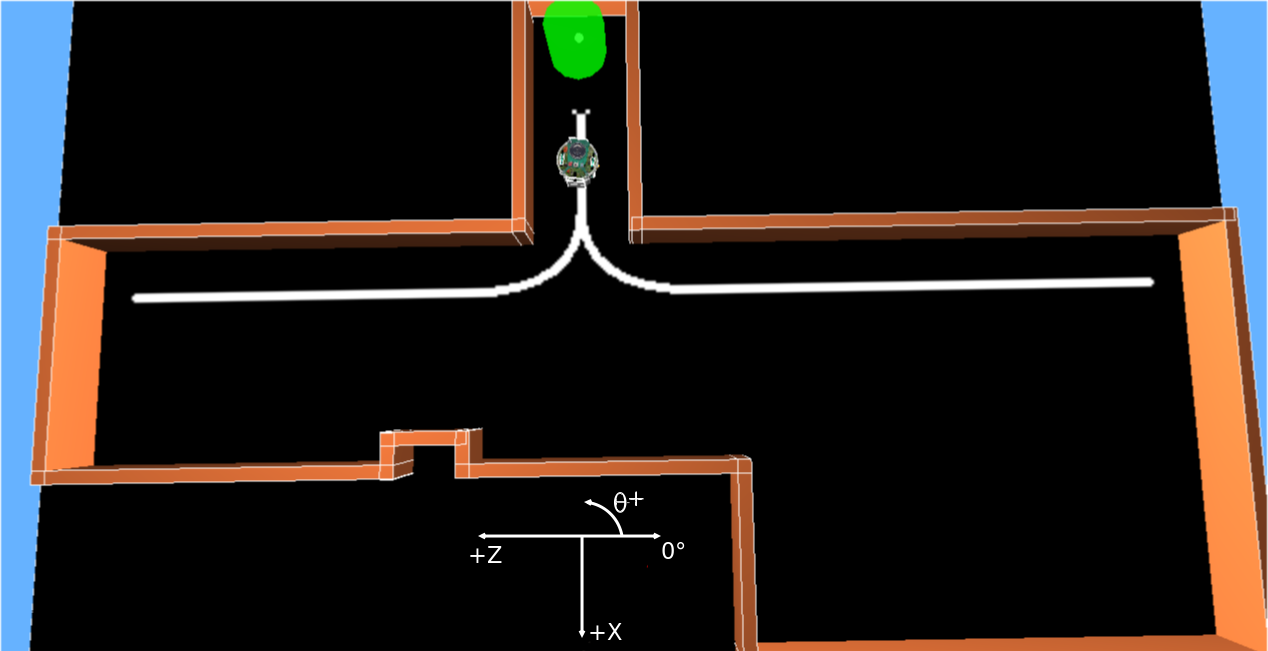
\includegraphics[scale=0.3]{comportamientos/arenafinal.png}
\caption{Arena de simulaci\'on y ejes de coordenadas}
\label{fig:arenafinal}
\end{center}
\end{figure}

\begin{figure}[htp]
\begin{center}
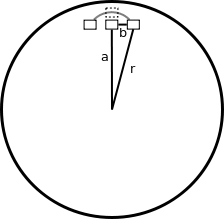
\includegraphics[scale=1.0]{comportamientos/floorSensors.png}
\caption{Disposici\'on de sensores de piso}
\label{fig:floorSensors}
\end{center}
\end{figure}

\subparagraph{Detalle del comportamiento}
La decisi\'on de dejar s\'olo dos l\'ineas, acompa\~nada por la elecci\'on de la ubicaci\'on de la
zona de descarga, nos facilit\'o la composici\'on de \'este comportamiento.
\\ Como se ve en la figura \ref{fig:arenafinal}, para ir a la l\'inea se debe girar hasta tener
un \'angulo de $\frac{\pi}{2}$ y luego ir hacia adelante.

%Describir la eleccion de las distancias de las lineas hacia las paredes

\subparagraph{Implementaci\'on del comportamiento}
El \emph{pseudo-codigo} de este comportamiento es sencillo, ya que
no requiere c\'alculos extras:

\begin{verbatim}
por cada paso
    angulo_actual = obtener_angulo_actual(odometria)
    si esta_en_un_entorno_de(angulo_actual,PI/2) entonces
        si angulo_actual > PI/2 && angulo_actual < 3PI/2 entonces
            giro_para_la_derecha
        sino
            giro_para_la_izquierda
        fin si
    sino
        voy_hacia_linea
    fin si
\end{verbatim}

Hicimos la verificaci\'on de que el \'angulo est\'e entre $\frac{\pi}{2}$ y $3\frac{\pi}{2}$
para evitar girar m\'as de $\pi$, girando a la izquierda o a la derecha dependiendo
cual sea el caso. Para ver esto m\'as claramente, veamos que sucediese si no estuviera:
\begin{verbatim}
    si esta_en_un_entorno_de(angulo_actual,PI/2) entonces
        giro_para_la_izquierda
    sino
\end{verbatim}
En el caso que el angulo actual sea $\pi$, el robot girar\'ia un total de $3\frac{\pi}{2}$
hasta llegar al \'angulo destino $\frac{\pi}{2}$, cuando en realidad girando para el sentido
contrario s\'olo tendr\'ia que girar $\frac{\pi}{2}$.
\\
Se puede observar en el c\'odigo usamos datos calculados por la odometr\'ia, en
este caso, la orientaci\'on actual del robot. El lector se podr\'ia preguntar:
``Si la odometr\'ia tiene la posici\'on actual del robot, ?`porqu\'e no se usaron los datos
de la misma para ir hacia la base?''. En principio, esto requiere que el robot tenga
conocimiento acerca de la ubicaci\'on de la base. Por otro lado, se hubiera tenido que utilizar
alg\'un algoritmo de \emph{Path Planning} para realizar el recorrido, algo que no
concuerda con la arquitectura elegida.
Es importante destacar el uso de datos calculados por la odometr\'ia porque si la misma
llega a tener un error grande, puede llevar a una activaci\'on err\'onea de comportamientos.
En la secci\'on \ref{odometry:problems} se puede ver la incidencia de un error grande de
la odometr\'ia en el comportamiento emergente del robot.

\paragraph{Entrar a l\'inea}
\label{enter_line}
\subparagraph{Detalle del comportamiento}

Para seguir la l\'inea, es necesario que primero el robot est\'e posicionado sobre ella
y alineado con la misma. Tambi\'en se necesita que la direcci\'on del robot sea la que
lo lleve hacia la zona de descarga, por lo que una vez en la l\'inea, el robot deber\'a
girar dependiendo de que lado se encuentre la misma (Ver figura \ref{fig:arenafinal}).

\subparagraph{Implementaci\'on del comportamiento}
\begin{verbatim}
    angulo_final = obtener_angulo_final(obtener_linea(odometria))
    tita = atan(dist_sens_piso_X,dist_sens_piso_Y)
    si ( esta_en_la_linea(sensor_piso(DERECHA)) ) entonces
        tita = -tita
    fin si
    si ( esta_en_la_linea(sensor_piso(MEDIO)) ) entonces
        tita = 0
    fin si

    si ( tita != 0 ) entonces
        girar(tita)
    fin si

    distancia_a_recorrer = dist_sens_piso_Y;
    si ( tita != 0 ) entonces
        distancia_a_recorrer = sqrt( dist_sens_piso_X^2 + dist_sens_piso_Y^2 )
    fin si

    recorrer(distancia_a_recorrer)

    angulo_actual = obtener_angulo(odometria)

    girar(normalizar(angulo_actual - angulo_final))
\end{verbatim}

%% Explicar el porque del primer giro - relacionarlo con la figura fig:floorSensors
El primer giro del robot es para lograr que el robot quede con el sensor de piso del medio
sobre la l\'inea. Como mostramos en la figura \ref{fig:floorSensorsStates}, en el caso (a) y (b)
el robot girar\'a de forma tal que llegue un caso parecido al (c) ya posiblemente el sensor del
medio no estar\'a en la l\'inea. Notar que si el sensor del medio est\'a en
la l\'inea, entonces el robot no gira, cualquiera sea el estado de los sensores de los costados.
El \'angulo que debe girar est\'a dado por $\theta = \arctan (\frac{Fss}{Fsd})$ (Ver figura
\ref{fig:floorSensors}) o $-\theta$ seg\'un cual sea el sensor que est\'e sobre la l\'inea.

\begin{figure}[htp]
\begin{center}
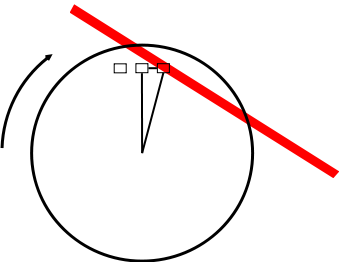
\includegraphics[scale=0.4]{comportamientos/floorSensorsLine.png}
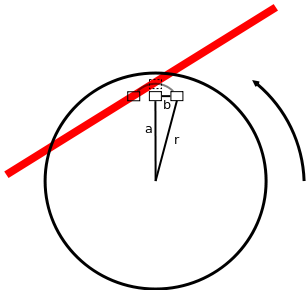
\includegraphics[scale=0.4]{comportamientos/floorSensorsLine1.png}
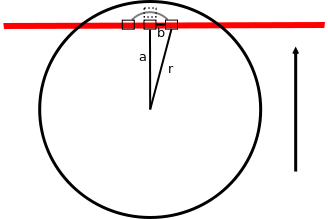
\includegraphics[scale=0.4]{comportamientos/floorSensorsLine2.png}
\caption{Posibles estados iniciales de entrar a la l\'inea}
\label{fig:floorSensorsStates}
\end{center}
\end{figure}


%% Explicar el porque del recorrido de la distancia - relacionarlo con la figura fig:floorSensors
Luego del posible giro para lograr que el sensor de piso del medio quede sobre la l\'inea, 
se recorre una distancia de $Fsd$, en el caso que el robot no haya girado anteriormente, o $Fsl$ en
el caso que s\'i lo haya hecho. El motivo de este trayecto es que el centro del robot quede
sobre la l\'inea, como muestra la figura \ref{fig:positioned}. De \'esta forma, s\'olo queda
girar nuevamente hacia el \'angulo que se quiera. Si la l\'inea es la izquierda, entonces el
robot deber\'a girar hasta que su orientaci\'on sea $0$, o $\pi$ en el caso que la l\'inea
sea la derecha.

\begin{figure}[htp]
\begin{center}
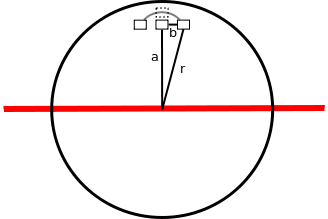
\includegraphics[scale=0.4]{comportamientos/floorSensorsLine3.png}
\caption{Centro del robot sobre la l\'inea y posibles giros}
\label{fig:positioned}
\end{center}
\end{figure}

\paragraph{Seguir l\'inea}
\label{follow_line}
Una vez que el robot est\'a posicionado y con el sensor del medio sobre la l\'inea,
s\'olo basta con seguirla para llegar hacia la zona deseada. \'Este comportamiento
es sencillo de desarrollar.

\subparagraph{Detalle del comportamiento}
Para lograr que el robot siga la l\'inea el objetivo es tratar de mantener s\'olo el
sensor del medio sobre la l\'nea. Entonces, basta con analizar que se debe hacer en los
siguientes casos:
\begin{enumerate}
	\item El sensor de la derecha est\'a sobre la l\'inea
	\item El sensor de la izquierda est\'a sobre la l\'inea
\end{enumerate}
En el primer caso, se debe lograr sacar el sensor de la derecha de la l\'inea,
describiendo un peque\~no arco hacia ese lado. El segundo caso es an\'alogo:
para sacar el sensor de la izquierda de la l\'inea se debe seguir una trayectoria
con un peque\~no \'angulo hacia la izquierda. 

\subparagraph{Implementaci\'on del comportamiento}
El \emph{pseudo-c\'odigo} es simple:
\begin{verbatim}
por cada paso
    veloc_izq = veloc_der = VELOC_SEGUIR_LINEA
    si ( esta_en_la_linea(sensor_piso(IZQUIERDA)) ) entonces
        veloc_izq *= ( 1 - FACTOR_DE_GIRO )
        veloc_der *= ( 1 + FACTOR_DE_GIRO )
    fin si
    si ( esta_en_la_linea(sensor_piso(DERECHA)) ) entonces
        veloc_izq *= ( 1 + FACTOR_DE_GIRO )
        veloc_der *= ( 1 - FACTOR_DE_GIRO )
    fin si
    poner_velocidades_en_ruedas(veloc_izq,veloc_der)
\end{verbatim}

\subsubsection{Descargar Basura}
\label{unload_garbage}
Una vez que el robot logr\'o llegar a la zona de descarga de basura, debe
descargarla. Para \'esto decidimos ubicar un servo en la parte trasera del robot,
con la misma idea del servo en la parte posterior utilizado para recolectar.

\paragraph{Detalle del comportamiento}
Para descargar la basura el robot debe posicionarse de forma tal que la compuerta
de descarga quede adyacente a la zona. Dado que para llegar a la misma el robot
sigui\'o la l\'inea, al finalizar va a estar orientado con un \'angulo en un
entorno de $\frac{\pi}{2}$, mirando la zona de descarga. Como el servo de descarga
se encuentra en la parte trasera, deber\'a realizar un giro para luego poder descargar
la basura.
\paragraph{Implementaci\'on del comportamiento}
\begin{verbatim}
    posicionarse()
    levantar(servo_trasero)
    recorrerdistancia(ANCHO_ROBOT)
    cerrar(servo_trasero)
\end{verbatim}

\subsubsection{Ir a base de recarga de bater\'ia}
\label{go_to_recharge}
Ayudados por la elecci\'on que tomamos de poner la zona de descarga de basura
muy cercana a la zona donde se recarga la bater\'ia, decidimos utilizar la
misma estrategia de seguir la l\'inea para llegar hacia la misma.
\\
La diferencia
entre ambos casos es el est\'imulo ante el cual se activan. En el caso de
ir a la zona de descarga, el est\'imulo proviene del sensor del dep\'osito
interno de basura que indica que el mismo est\'a lleno. En el caso de ir
a la base de recarga de bater\'ia, el est\'imulo para la activaci\'on depende
de los valores de dos sensores de bater\'ia que indican bater\'ia baja:
\begin{itemize}
	\item El sensor de la bater\'ia del robot, de donde se alimentan los sensores,
			actuadores y motores.
	\item El sensor de la computadora que corre el controlador.
\end{itemize}

\subsubsection{Cargar Bater\'ia}
\label{recharge_battery}
\paragraph{Detalle del comportamiento}
\paragraph{Implementaci\'on del comportamiento}
\begin{verbatim}
    posicionarse()
    mientras( bateria_no_llena(BATERIA_ROBOT)
            o bateria_no_llena(BATERIA_PC) ) hacer

        esperar()
    fin mientras
\end{verbatim}

\begin{comment}

\subsubsection{Recalibrarse}
\label{recalibrate}
\paragraph{Detalle del comportamiento}
\paragraph{Implementaci\'on del comportamiento}

\end{comment}

\subsubsection{Evitar Obst\'aculos}
\label{avoid_obstacles}
\emph{Evitar obst\'aculos} es uno de los comportamientos con mayor jerarqu\'ia
en la arquitectura que elegimos. Su nivel se debe a la importancia que tiene
en un ambiente estructurado pero din\'amico como es el elegido. El objetivo
del robot es facilitar una tarea, sin entorpecer el tr\'ansito de personas.
\\
\paragraph{Detalle del comportamiento}
Para lograr tener conocimiento sobre la proximidad de un obst\'aculo, utilizamos
sensores de proximidad explicados en \ref{sensores de proximidad}.
Dependiendo de la proximidad sensada por un sensor, el robot deber\'a alejarse
de ese lado para evitar un posible choque. La activaci\'on del comportamiento
depender\'a entonces de un valor menor del sensor que haga que la distancia hacia
un obst\'aculo lleve al robot a quedarse estancado o le imposibilite moverse.
\paragraph{Implementaci\'on del comportamiento}
La implementaci\'on de \'este comportamiento la hicimos utilizando una red neuronal
sin capas ocultas 
(ver figura \ref{fig:redN}) usando los sensores de distancia como entradas y las
2 neuronas de salida indicando los valores a ser seteados a los motores de las ruedas.
\\
Notar que hay conexiones tanto inhibitorias como excitatorias. Como es de esperarse,
ambos sensores traseros ( 4 y 5 ) exitan a ambos motores. Distinto es el caso de los
sensores del lado izquierdo ( 5, 6 y 7 ) que exitan el motor ubicado de su lado e
inhiben el motor del lado opuesto, de forma tal que el robot gire para el lado
opuesto de la ubicaci\'on de los sensores. La misma idea se sigue con los sensores
( 0, 1 y 2 ) ubicados en el costado derecho del robot.
\\
Luego de entrenar la red, obtuvimos los siguientes valores para los pesos de la
misma:

\begin{table}[ht]
	\begin{center}
		\begin{tabular}{ | c | c | c | c | c | c | c | c | c | }
			\hline 
			Rueda & $W_0$ & $W_1$ & $W_2$ & $W_3$ &  $W_4$ & $W_5$ & $W_6$ & $W_7$ \\
			\hline\hline
			Izquierda & -0.9 & -0.85 & -0.2 & 0.6 & 0.5 & 0.35 & 0.8 & 0.6 \\
			\hline
			Derecha & 0.9 & 0.85 & 0.2 & 0.6 & 0.5 & -0.35 & -0.8 & -0.6 \\
			\hline
		\end{tabular}
	\end{center}
	\label{pesos_obstaculo} 
	\caption{Asignaci\'on de pesos para evitar obst\'aculos}
\end{table}
Se puede ver que los pesos que influyen en el motor de una rueda influyen
con igual fuerza pero distinto signo en el motor de la rueda contraria.
\\
Este comportamiento, en \emph{pseudo-codigo} puede verse como:
\begin{verbatim}
por cada paso
    veloc_izq = suma( coeficiente(RUEDA_IZQ)(SENSOR_I) * VALOR(SENSOR_I) )
    veloc_izq *= FACTOR_DE INCIDENCIA
    veloc_der = suma( coeficiente(RUEDA_DER)(SENSOR_I) * VALOR(SENSOR_I) )
    veloc_der *= FACTOR_DE INCIDENCIA
    poner_velocidades_en_ruedas(veloc_izq,veloc_der)
\end{verbatim}

\begin{figure}[htp]
\begin{center}
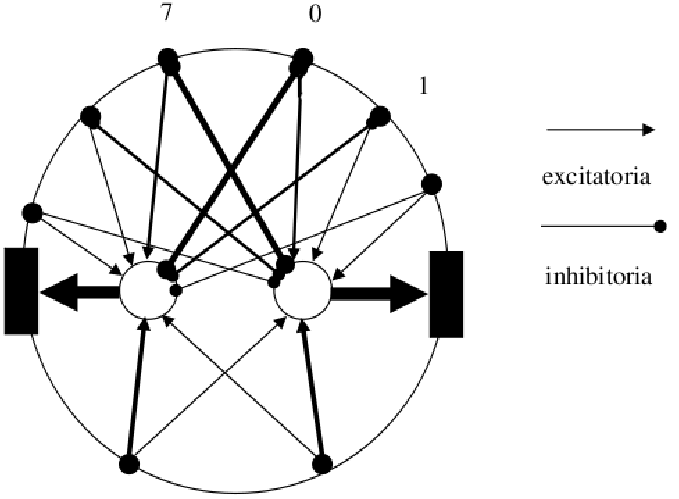
\includegraphics[scale=0.4]{comportamientos/red.png}
\caption{Red neuronal entre los sensores de distancia y los motores}
\label{fig:redN}
\end{center}
\end{figure}

\subsubsection{Salir de situaciones no deseadas}
\label{out_of_unwanted_situations}
\emph{Salir de situaciones no deseadas} surgi\'o como un comportamiento
para ayudar al objetivo de la autonom\'ia del robot. A medida que fuimos
corriendo las simulaciones, observamos que hab\'ia situaciones donde corr\'ia
peligro la autonom\'ia del robot. Un ejemplo de estas situaciones es el caso
donde se ``activan mutuamente'' entre dos comportamientos.
\\
Para ver esto m\'as claramente, supongamos dos comportamientos $A$ y $B$ con
nivel en la jerarqu\'ia $N(A)$ y $N(B)$, siendo $N(A) > N(B)$. Si la respuesta
a un est\'imulo de $A$ lleva a la activaci\'on de $B$ y a la desactivaci\'on de $A$
y luego la respuesta de $B$ lleva a la activaci\'on de $A$, podr\'ia llegar a
entrarse en un ciclo si es que esta situaci\'on se da por un tiempo prolongado.
El mayor peligro para la autonom\'ia se corre cuando $A$ es el comportamiento
de \emph{evitar obst\'aculos} y $B$ es el comportamiento de \emph{ir a zona
de recarga de bater\'ia} ya que el robot podr\'ia terminar qued\'andose sin
bater\'ia en ese ciclo.
\paragraph{Detalle del comportamiento}
Las situaciones no deseadas se dan la mayor\'ia de los casos cuando un comportamiento
hace girar al robot hacia un lado y el otro comportamiento hacia el lado contrario,
aproximadamente en la misma magnitud. \'Esto quiere decir que la posici\'on del
robot se mantiene alrededor de un punto por un per\'iodo prolongado de tiempo,
por lo que decidimos tomar este hecho como est\'imulo para la activaci\'on de este
comportamiento.
\\
La respuesta del comportamiento es, entonces, girar un \'angulo que cambie
la direcci\'on del robot y adem\'as, que la suma de esa magnitud no sea peri\'odica.
\'Esta \'ultima condici\'on se pide por el siguiente escenario:
\begin{itemize}
	\item Los comportamientos $A$ y $B$ se ``activan mutuamente'' cuando la orientaci\'on
			del robot es $0$.
	\item Los comportamientos $C$ y $D$ se ``activan mutuamente'' cuando la orientaci\'on
			del robot es $\pi$.
	\item La respuesta de \emph{salir de situaciones no deseadas} es girar un \'angulo $\pi$.
\end{itemize}

\paragraph{Implementaci\'on del comportamiento}
\begin{verbatim}
    angulo_actual = obtener_angulo_actual(odometria)
    nuevo_angulo = angulo_actual + ANGULO_A_SUMAR
    girar(nuevo_angulo)
\end{verbatim}

